\setAuthor{}
\setRound{lõppvoor}
\setYear{2019}
\setNumber{G 8}
\setDifficulty{8}
\setTopic{TODO}

\prob{Kärbes}
Kärbes lendab läätse peateljega paralleelselt, teljest kaugusel $a$, läätse suunas konstantse kiirusega $v$ alustades suurest kaugusest ja lõpetades läätse juures. Läätse fookuskaugus on $f$. Milline on selle lennu jooksul kärbse minimaalne kiirus tema kujutise suhtes? 

\hint

\solu
Kui kärbes liigub mööda joonisel näidatud horisontaalset sirget, mis lõikub läätsega punktis A ja alustab liikumist väga kaugelt, siis kärbse kujutis liigub mööda kaldjoont, mis läbib punkti A ja fookust F (sest sirge kujutis on sirge ja need kaks sirget lõikuvad läätse tasandis) ning alustab liikumist punktist F eemaldudes alguses väga aeglaselt. Kujutise kiirus kasvab monotoonselt kuni jõuab lõpmatusse hetkel, mil kärbes läbib fokaaltasandi. Seega, kui kärbse kiirust kujutab horisontaalne vektor $v$ parempoolsel joonisel, siis kujutise kiiruse vektor erinevatel ajahetkedel on kujutatud kaldus olevate vektoritena $u$. On ilmne, et nende kahe vektori vahe $w$ on minimaalne siis, kui vektor $w$ on risti vektoriga $u$. Seega saame $u_{\min}=v\sin\alpha$. Kolmnurga $OAF$ põhjal $\sin\alpha=a/\sqrt{a^2+f^2}$ ning $u_{\min}=va/\sqrt{a^2+f^2}$.\\

\begin{center}
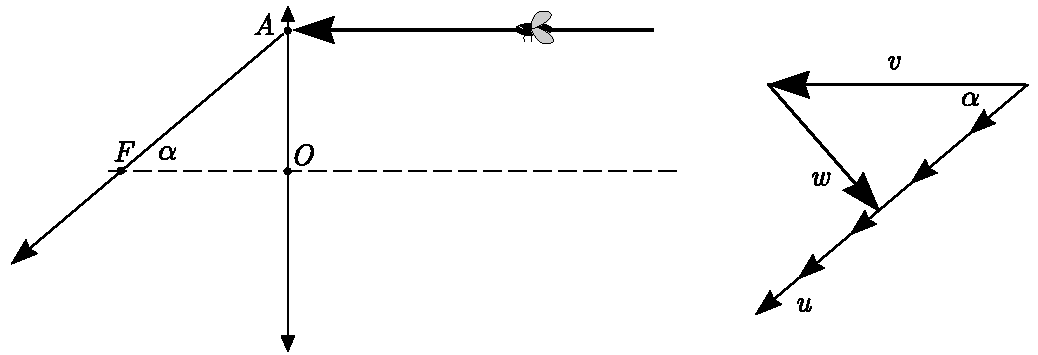
\includegraphics[scale=0.7]{2019-v3g-08-yl.pdf}
\end{center}
\probend